

% ===========================
\chapter{Ergebnis}
\label{ergebnis}
% ===========================

In diesem Kapitel werden die Ergebnisse der trainierten \acp{KNN} aus Abschnitt \ref{umsetzung_training_architektur} mit den Parametern aus Abschnitt \ref{umsetzung_training_experimente} vorgestellt. Jede Architektur wird mit einer Maximalanzahl von 100 Epochen trainiert. Aufgrund der Regularisierungsmethode Early Stopping wird diese Anzahl jedoch nie erreicht. Das Training bricht jeweils ab, wenn sich die Klassifizierungsgenauigkeit der Validierungsdaten innerhalb von 20 Epochen nicht um mindestens 0,01 verbessert. Nach Abbruch werden jeweils die Gewichte der Epoche mit der höchsten Genauigkeit wiederhergestellt. 

In Abschnitt \ref{ergebnis_parameter} wird die Genauigkeit der jeweiligen Netzarchitekturen bei der Klassifizierung der realen Testdaten und die Anzahl der trainierten Epochen hinsichtlich der unterschiedlichen Parameter aus Abschnitt \ref{umsetzung_training_experimente} verglichen. Danach wird in Abschnitt \ref{ergebnis_synth_vs_real} die Genauigkeit der Klassifizierung zwischen realen und synthetischen Testdaten untersucht. Im Anschluss werden in Abschnitt \ref{ergebnis_szenarien} die Unterschiede bei der Erkennung von verschiedenen Klassen erörtert.


% ===========================
\section{Variation der Parameter}
\label{ergebnis_parameter}
% ===========================

In diesem Abschnitt werden die Unterschiede der verschiedenen Architekturen aus Abschnitt \ref{umsetzung_training_architektur} noch einmal kurz aufgegriffen und dann die dazugehörigen Ergebnisse vorgestellt. Die Ergebnisse sind in Tabelle \ref{tab_ergebnis_real} zusammengefasst.

\begin{table}[h]
\small
\centering
\def\arraystretch{1.4}
\begin{tabular}{c p{3cm} c c}
\textbf{Architektur} & \textbf{Beschreibung} & \textbf{Genauigkeit} & \textbf{Epochen} \\
\hline
A & Inception-V3 & 0,73 & 4 \\
\hline
B & Inception-V3 \newline Dropout & 0,64 & 1 \\
\hline
C & Xception & 0,54 & 1 \\
\hline
D & Xception \newline Dropout & 0,48 & 9 \\
\hline 
E & Inception-V3 \newline LSTM & 0,36 & 80 \\
\hline
F & Inception-V3 \newline LSTM \newline Dropout & 0,95 & 12 \\
\hline
G & Xception \newline LSTM & 0,38 & 26 \\
\hline
H & Xception \newline LSTM \newline Dropout & 0,28 & 3 \\
\hline
\end{tabular}
\caption{Ergebnisse der verschiedenen Architekturen bei der Klassifizierung der realen Testdaten}
\label{tab_ergebnis_real}
\end{table}

% ===========================
\subsubsection{Prinzip der Klassifizierung}
% ===========================

Bei der Klassifizierung wird in dieser Arbeit zwischen \acp{KNN} für die Erkennung von einzelnen Bildern und für die Erkennung von 3-Sekunden-Videos mit jeweils 15 Bildern unterschieden. Die detaillierten Architekturen sind in Abschnitt \ref{umsetzung_training_architektur} vorgestellt.

Insgesamt wurde die höchste Genauigkeit bei der Klassifizierung der realen Testdaten von 0,95 mit der Architektur F für Videoerkennung erreicht. Dieses Ergebnis ist auch in Abbilder \ref{fig_cm_v3_lstm_d_real} in der Konfusionsmatrix (engl. confusion matrix) dargestellt. Gleichzeitig wurde auch die niedrigste Genauigkeit mit der Architektur H für Videoerkennung erreicht. Architekturen für die reine Bilderkennung erreichen Genauigkeiten zwischen 0,48 (Architektur D) und 0,73 (Architektur A). Damit erzielen diese Architekturen Ergebnisse mit weniger Varianz im Vergleich zu den anderen Architekturen.

\begin{figure}[h]
\centering
{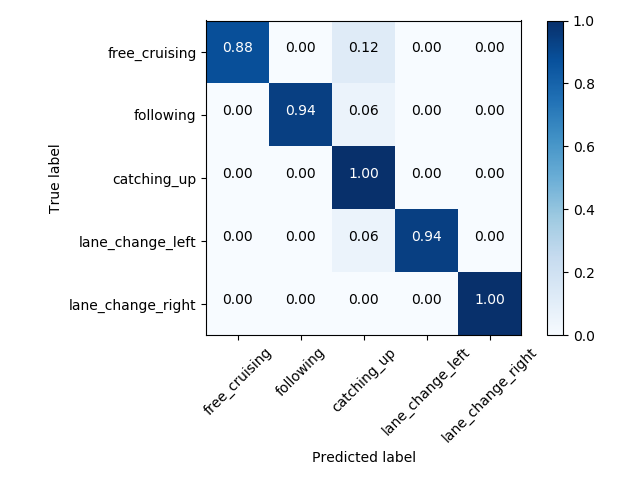
\includegraphics[scale=0.7]{cm_v3_lstm_d_real.png}}
\caption{Konfusionsmatrix der Klassifizierung von realen Testdaten mit der Architektur F (Inception-V3, \ac{LSTM}, Dropout)}
\label{fig_cm_v3_lstm_d_real}
\end{figure}

% ===========================
\subsubsection{\aclp{CNN}}
% ===========================

Der Vergleich zwischen den zwei \ac{CNN}-Architekturen Inception-V3 und Xception zeigt ein klares Bild. In drei von vier Fällen kann die Architektur mit der Inception-V3-Architektur bessere Ergebnisse erzielen. Der Unterschied ist dabei zwischen 0,16 und 0,67 bei der Genauigkeit. Nur die Architektur G erzielt eine höhere Genauigkeit als Architektur E mit einem Unterschied von 0,02. Dieser Unterschied überrascht, da die Xception-Architektur in anderen Arbeiten \cite{chollet2017xception} höhere Genauigkeiten bei der Klassifizierung von Bildern erreicht hat.

% ===========================
\subsubsection{Regularisierung mit Dropout}
% ===========================

Es ist auffällig, dass die Architekturen für Videoklassifizierung mit Dropout in der vorletzten Fully-Connected-Schicht deutlich bessere Ergebnisse erzielen können im Vergleich zu denselben Architekturen ohne Dropout. Im Gegensatz dazu erzielen die Architekturen für die Erkennung einzelner Bilder die bessere Genauigkeit ohne Dropout.

Eine mögliche Erklärung dafür könnte die Komplexität der Architekturen mit \ac{LSTM}-Schicht sein. Diese Architekturen haben mehr trainierbare Parameter und sind daher anfälliger für eine Überanpassung \cite{hinton2012improving}. Regularisierung mit Dropout kann die Komplexität reduzieren und führt zu höheren Genauigkeiten. Die Architekturen mit reinen \acp{CNN} sind weniger komplex und daher hat Dropout keine oder eine negative Auswirkung auf das Ergebnis.

% ===========================
\subsubsection{Anzahl der Epochen}
% ===========================

Es lässt sich beobachten, dass die Architekturen für die Klassifizierung von Videos mit bis zu 80 Epochen deutlich mehr Trainingsschritte benötigen als die Architekturen für reine Bilderkennung. Eine mögliche Erklärung dafür ist, dass reine \acp{CNN} eine weniger komplexe Architektur und weniger Parameter haben als die Architekturen mit einer \ac{LSTM}-Schicht. Mehr Gewichte, die angepasst werden können, bedeutet eine höhere Komplexität und dementsprechend mehr Trainingszeit.

Bei den Architekturen für die Klassifizierung von Videos reduziert Dropout die Anzahl der benötigten Epochen drastisch. Eine mögliche Erklärung ist die hohe Komplexität dieser Architekturen, die mit Dropout reduziert werden kann \cite{hinton2012improving}.

Zu den Unterschieden der Trainingszeiten zwischen der Inception-V3- und der Xception-Architektur lässt sich in dieser Arbeit keine eindeutige Aussage treffen. Die benötige Epochenanzahl bei beiden Architekturen variiert sehr stark.

% ===========================
\section{Synthetische und reale Testdaten}
\label{ergebnis_synth_vs_real}
% ===========================

In diesem Abschnitt werden die Unterschiede der Genauigkeiten bei der Klassifizierung zwischen realen und synthetischen Testdaten untersucht. Die Ergebnisse sind in Tabelle \ref{tab_ergebnis_synth} zusammengefasst. Es ist nicht überraschend, dass die Genauigkeiten bei der Klassifizierung von synthetischen Testdaten überwiegend deutlich höher ist, weil die \acp{KNN} mit circa 95\% synthetischer und nur 5\% realer Daten trainiert wurden. Das bestätigt auch die Ergebnisse der vorangegangenen Arbeit, die in Abschnitt \ref{grundlagen_nn_synthetisch} diskutiert werden. 

Es ist auffällig, dass die Klassifizierung von einzelnen synthetischen Bildern mit der Xception Architektur niedriger ist als die Klassifizierung von realen Testbildern. Aktuell hat der Autor keine Erklärung hierfür. Dieses Ergebnis kann als Ausgangspunkt für weitere Arbeiten dienen.

\begin{table}[h]
\small
\centering
\def\arraystretch{1.4}
\begin{tabular}{c p{3cm} c c}
\textbf{Architektur} & \textbf{Beschreibung} & \textbf{Genauigkeit} & \textbf{Genauigkeit} \\
 & & \textbf{Reale Testdaten} & \textbf{Synthetische Testdaten} \\
\hline
A & Inception-V3 & 0,73 & 0,96 \\
\hline
B & Inception-V3 \newline Dropout & 0,64 & 0,96 \\
\hline
C & Xception & 0,54 & 0,2 \\
\hline
D & Xception \newline Dropout & 0,48 & 0,36 \\
\hline 
E & Inception-V3 \newline LSTM & 0,36 & 0,94 \\
\hline
F & Inception-V3 \newline LSTM \newline Dropout & 0,95 & 0,99 \\
\hline
G & Xception \newline LSTM & 0,38 & 0,99 \\
\hline
H & Xception \newline LSTM \newline Dropout & 0,28 & 0,67 \\
\hline
\end{tabular}
\caption{Ergebnisse der Klassifizierung von synthetischen und realen Testdaten}
\label{tab_ergebnis_synth}
\end{table}


% ===========================
\section{Genauigkeit der einzelnen Szenarien}
\label{ergebnis_szenarien}
% ===========================

Die Betrachtung Klassifizierungsgenauigkeiten der einzelnen Klassen ergibt kein eindeutiges Bild. Bei verschiedenen Architekturen werden verschiedene Szenen besser oder schlechter erkannt. Hervorzuheben ist, dass es deutliche Unterschiede gibt, diese aber keinem erkennbaren Muster folgen. Eine Übersicht der Genauigkeit der Klassifizierung von realen Testdaten auf der Ebene von Szenarienklassen ist in Tabelle \ref{tab_ergebnis_szenarien} dargestellt.

\begin{table}[h]
\small
\centering
\def\arraystretch{1.4}
\begin{tabular}{c c c c c c}
\textbf{Architektur} & \textbf{Free} & \textbf{Following} & \textbf{Catching} & \textbf{Lane change} & \textbf{Lane change} \\
 & \textbf{cruising} & & \textbf{up} & \textbf{left} & \textbf{right} \\
\hline
A & 0,65 & 0,76 & 1,00 & 0,35 & 0,88 \\
B & 0,94 & 0,47 & 0,88 & 0,29 & 0,59 \\
C & 0,76 & 0,94 & 0,94 & 0,00 & 0,06 \\
D & 0,00 & 0,82 & 0,82 & 0,76 & 0,00 \\
E & 0,59 & 0,47 & 0,41 & 0,06 & 0,29 \\
F & 0,88 & 0,94 & 1,00 & 0,94 & 1,00 \\
G & 0,47 & 0,06 & 0,18 & 0,59 & 0,06 \\
H & 0,12 & 0,00 & 0,00 & 0,65 & 0,65 \\
\hline
\textbf{Durchschnitt} & 0,55 & 0,57 & 0,65 & 0,46 & 0,44 \\
\hline
\end{tabular}
\caption{Genauigkeit der Klassifizierung von realen Testdaten auf der Ebene von Szenarienklassen}
\label{tab_ergebnis_szenarien}
\end{table}













